\section{Experimental Data and Analysis}
\label{sec:data}

We generated several problem suites with \fuzzer{} that made one
solver perform poorly, but not others. These suites are
\theSuites{}. Figure~\ref{fig:cvc-hard} shows the suites that were
uniquely difficult for \cvc{}. Figure~\ref{fig:z3str3-hard} shows the
suites that were uniquely difficult for \us{}. All experiments were
run in series on the same Linux computer, with a timeout of 15
seconds. \todo{Specify CPU, memory}

\begin{figure}[h]
    \begin{subfigure}{.5\textwidth}
        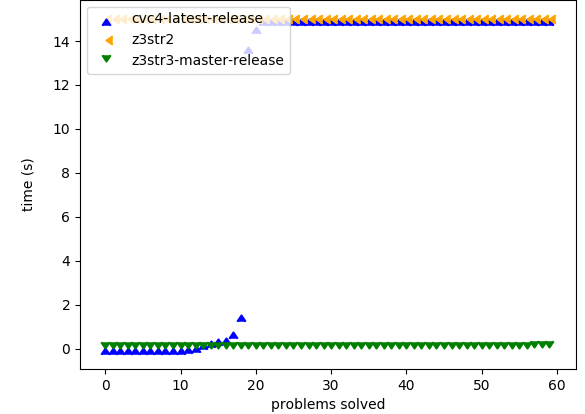
\includegraphics[width=\textwidth]{data/graphs/concats-extracts-small.png}
        \caption{Performance on concats-extracts-small}
        \label{fig:concats-extracts-small}
    \end{subfigure}
    \begin{subfigure}{.5\textwidth}
        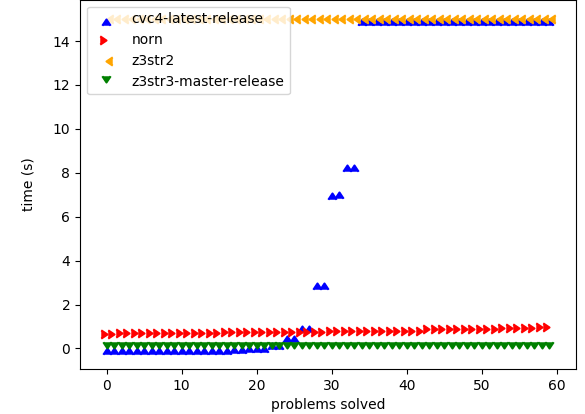
\includegraphics[width=\textwidth]{data/graphs/different-prefix.png}
        \caption{Performance on different-prefix}
        \label{fig:different-prefix}
    \end{subfigure}
    \caption{Problems hard for \cvc{}}
    \label{fig:cvc-hard}

    \begin{subfigure}{.5\textwidth}
        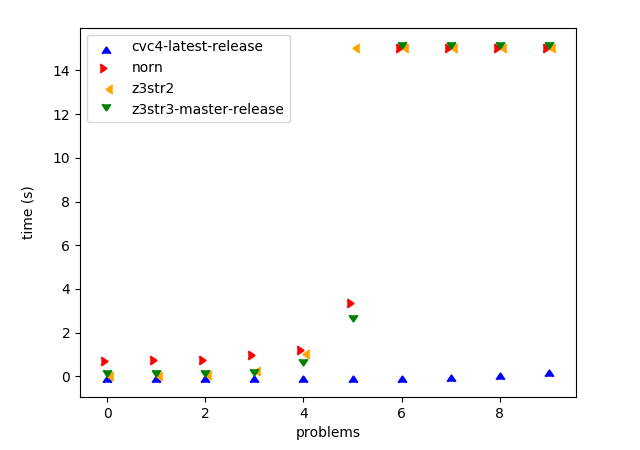
\includegraphics[width=\textwidth]{data/graphs/concats-balanced.png}
        \label{fig:concats-balanced}
        \caption{Performance on concats-balanced}
    \end{subfigure}
    \begin{subfigure}{.5\textwidth}
        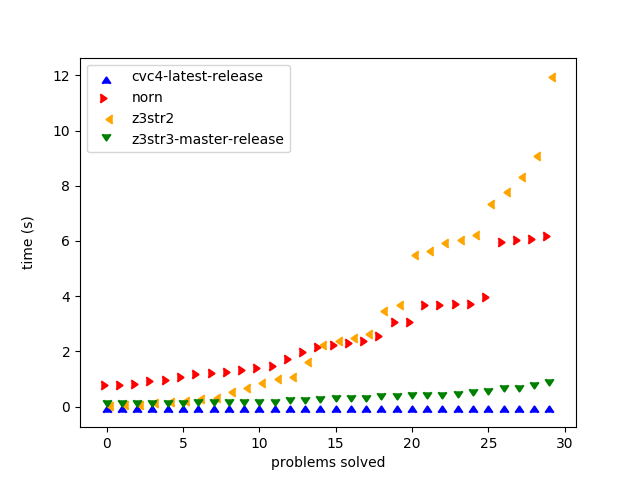
\includegraphics[width=\textwidth]{data/graphs/concats-small.png}
        \label{fig:concats-small}
        \caption{Performance on concats-small}
    \end{subfigure}
    \caption{Problems hard for \us{}}
    \label{fig:z3str3-hard}
\end{figure}

\subsubsection{Usefulness to \us{}: A Case Study}

We found a number of performance-related issues and opportunities for
new heuristics in \us{} thanks to \fuzzer{}. For example, the
instances in the \texttt{concats-big} suite generated by \fuzzer{}
helped us discover a missing heuristic. In particular, \us{} didn't
make full use of the solving context (e.g. some terms are empty
strings) to simplify the concatenations of a long list of string terms
before trying to reason about the equivalences among subterms. \us{}
therefore introduced a large number of unnecessary intermediate
variables and propagations. As an immediate consequence of
testing \us{} on \texttt{concats-big} benchmarks, we were able to
identify the factors common to these instances and rapidly formulate a
hypothesis as to why they were performing poorly.

%% %VG: this subsection is not needed in the paper
%% \noindent{\textbf{Defects discovered and fixed in \us{}:}} The first
%% issue we found caused \us{} to perform poorly when equivalence classes
%% of arithmetic terms were very large (e.g. the lengths of many strings
%% were equal to 0). This issue was detected by the \texttt{Concats}
%% problem suite. The slowdown was caused by a loop over terms in the
%% same equivalence class to search for an integer constant. The fix was
%% to check the root of the equivalence class for the integer constant,
%% as Z3 makes ``interpreted terms'' (e.g. constants) the root of
%% equivalence classes whenever possible. The second issue, which was
%% exposed by the \texttt{Lengths} suite, caused \us{} to perform poorly
%% when a variable has a large length constraint.  The slowdown was
%% caused by the solver performing a search for a satisfying length even
%% when the input formula explicitly constrained the exact length of a
%% string term.  The fix was to check whether the integer solver had
%% already assigned a length value before searching for length, and skip
%% the search if this was the case.

%% In order to improve the efficiency of any solver, discovering new
%% heuristics is crucial.  As an illustrative example, consider the
%% problem of how the a string solver may detect conflicting
%% constraints. A string solver that gradually propagates
%% (dis)equalities discovered along the way will eventually detect a
%% conflict.  However, in many scenarios, a conflict can be discovered
%% ``early'' before trying to figure out the relationships among
%% subterms and propagating the facts.  The benefits of this eager
%% approach are clear: this saves the effort of reasoning about
%% subterms and propagating observations, as a conflict will
%% eventually be reached in either case, forcing conflict analysis and
%% a backjump.  As reported in existing works, heuristics of this form
%% usually lead to significant improvements.  However, the process of
%% discovering such heuristics is extremely challenging, as they are
%% usually learned from a class of examples whose commonalities are
%% not always obvious or immediately indicative of such
%% inefficiencies.
